The goal of this task was to rectify a \(300 \times 400\) grayscale image \(A\) (``\texttt{homework6.pgm}'') and generate a \(300 \times 370\) output image \(B\) by applying a projective transformation \(h\). This transformation maps the quadrilateral defined by the following points in image \(A\):

\[
\begin{aligned}
p_1 &= (244, 263), \\
p_2 &= (238, 353), \\
p_3 &= (199, 350), \\
p_4 &= (201, 262)
\end{aligned}
\]

to the following points in image \(B\):

\[
\begin{aligned}
q_1 &= (232, 216), \\
q_2 &= (232, 311), \\
q_3 &= (197, 311), \\
q_4 &= (197, 216)
\end{aligned}
\]

To accomplish this, the inverse of the homography matrix \(H\) that maps destination points \(q_i\) to source points \(p_i\) was computed using \texttt{cv2.findHomography}. This inverse transformation was then used to warp the original image using bilinear interpolation via \texttt{cv2.warpPerspective}, thereby generating image \(B\). The output image has a fixed resolution of \(300 \times 370\) as required.

Resulting image:
\begin{figure}[H]
    \centering
    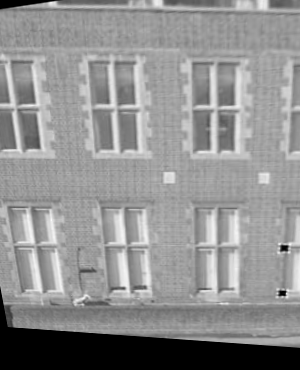
\includegraphics[width=0.5\textwidth]{../Images/homework6.png}
    \caption{Rectified image \(B\) with a resolution of \(300 \times 370\)}
\end{figure}
